% Proposta A: Figura 4 do Cap. I só com o conceito (15/11/2026). Fora do TG.
\documentclass[11pt,border=2pt]{standalone}
% Estilo comum às propostas (o mesmo da Figura 4 atual, tg/figuras/fig05-fluxo-arima.tex)
\usepackage[T1]{fontenc}
\usepackage[utf8]{inputenc}
\usepackage{mathptmx}
\usepackage{tikz}
\usetikzlibrary{arrows.meta,positioning,calc,shapes.geometric,decorations.pathreplacing}
\tikzset{
  seta/.style={-{Stealth[length=2.2mm]}, semithick},
  caixa/.style={rectangle, draw, semithick, fill=gray!10, rounded corners=2pt,
                align=center, minimum width=58mm, minimum height=9mm, font=\small},
  caixap/.style={caixa, minimum width=32mm},
  decisao/.style={diamond, draw, semithick, fill=white, aspect=2.6, align=center,
                  inner sep=1pt, font=\small},
  dado/.style={trapezium, trapezium left angle=75, trapezium right angle=105, draw,
               semithick, fill=white, align=center, minimum height=9mm, font=\small,
               trapezium stretches body},
  rotulo/.style={font=\footnotesize\itshape, align=center},
  exemplo/.style={font=\footnotesize, text=gray!70!black, align=left},
}

\begin{document}
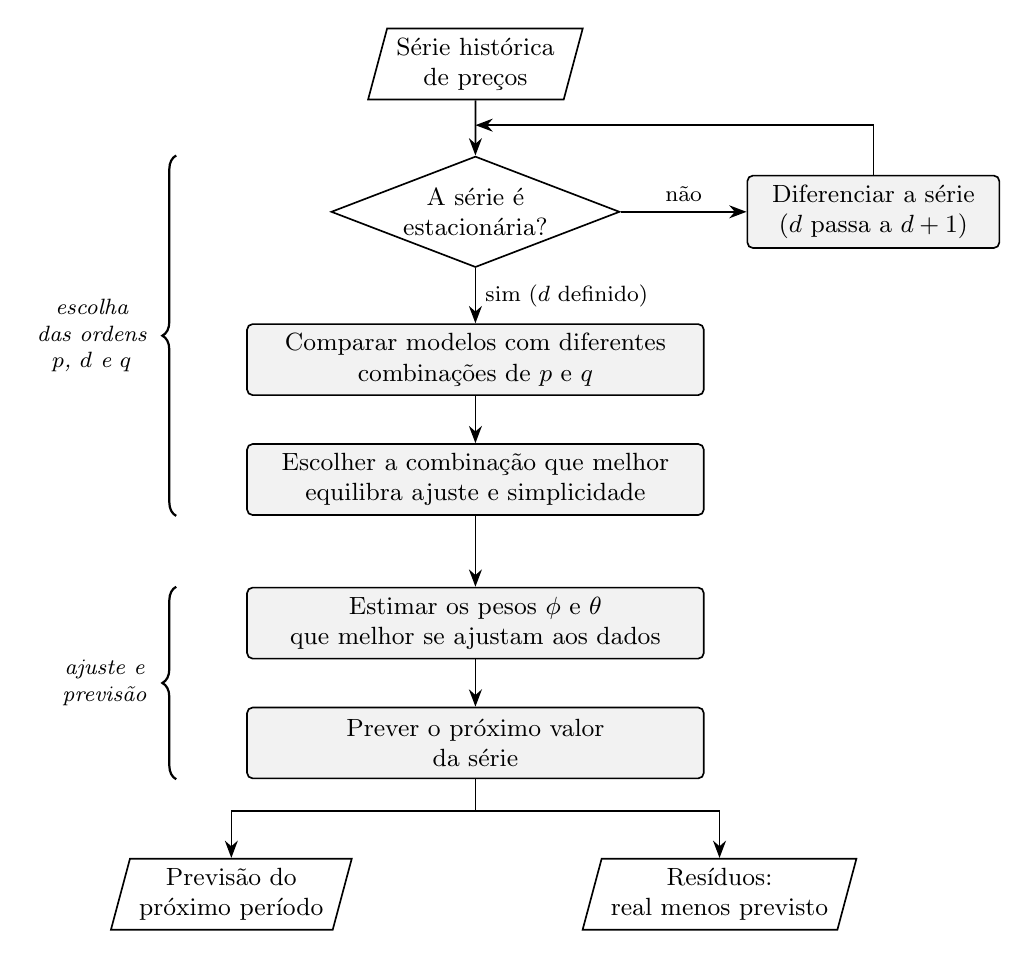
\begin{tikzpicture}[node distance=6mm]
  \node[dado] (ent) {Série histórica\\de preços};
  \node[decisao, below=7mm of ent] (est) {A série é\\estacionária?};
  \node[caixap, right=16mm of est] (dif) {Diferenciar a série\\($d$ passa a $d+1$)};
  \node[caixa, below=7mm of est] (comp) {Comparar modelos com diferentes\\combinações de $p$ e $q$};
  \node[caixa, below=of comp] (esc) {Escolher a combinação que melhor\\equilibra ajuste e simplicidade};
  \node[caixa, below=9mm of esc] (pesos) {Estimar os pesos $\phi$ e $\theta$\\que melhor se ajustam aos dados};
  \node[caixa, below=of pesos] (prev) {Prever o próximo valor\\da série};
  \node[dado, below=10mm of prev, xshift=-31mm] (sai) {Previsão do\\próximo período};
  \node[dado, below=10mm of prev, xshift=31mm] (res) {Resíduos:\\real menos previsto};

  \coordinate (volta) at ($(ent.south)!0.45!(est.north)$);
  \draw[seta] (ent) -- (est);
  \draw[seta] (est) -- node[above, font=\footnotesize]{não} (dif);
  \draw[seta] (dif.north) |- (volta);
  \draw[seta] (est) -- node[right, font=\footnotesize]{sim ($d$ definido)} (comp);
  \draw[seta] (comp) -- (esc);
  \draw[seta] (esc) -- (pesos);
  \draw[seta] (pesos) -- (prev);
  \draw[seta] (prev.south) -- ++(0,-4mm) -| (sai.north);
  \draw[seta] (prev.south) -- ++(0,-4mm) -| (res.north);

  \draw[decorate, decoration={brace, amplitude=5pt, mirror}, thick]
    ([xshift=-38mm]est.north) -- ([xshift=-38mm]esc.south)
    node[midway, left=7pt, rotulo]{escolha\\das ordens\\$p$, $d$ e $q$};
  \draw[decorate, decoration={brace, amplitude=5pt, mirror}, thick]
    ([xshift=-38mm]pesos.north) -- ([xshift=-38mm]prev.south)
    node[midway, left=7pt, rotulo]{ajuste e\\previsão};
\end{tikzpicture}
\end{document}
